% calculus:x10
\bigskip
\begin{question}
  \hspace*{\fill} [Note maximale: 6]\par
  \noindent Une fonction $f$ est définie pour $-4 \le x \le 3$. La représentation graphique de $f$ est donnée ci-dessous.\par
  \medskip
  \begin{center}
    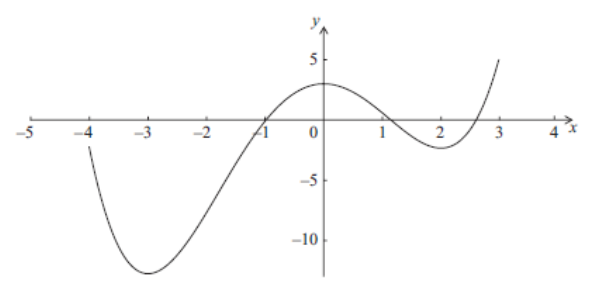
\includegraphics[scale=0.25]{temp_polynom_minus4_to_3}\par
  \end{center}
  \noindent La représentation graphique présente un maximum relatif en $x = 0$ et des minimums relatifs en $x = -3$ et $x = 2$.\par
  \medskip
  (a) Donnez les abscisses à l’origine de la représentation graphique de la fonction dérivée, $f^\prime$.\hspace*{\fill} [2]\par
  \medskip
  (b) Donnez toutes les valeurs de $x$ pour les quelles $f^\prime(x)$ est positive.\hspace*{\fill} [2]\par
  \medskip
  (c) Au point $D$ sur la représentation graphique de $f$, l’abscisse est $-0,5$.\par
  \hspace{2em} Expliquez pourquoi $f^{\prime\prime}(x) < 0$ en $D$.\hspace*{\fill} [2]\par
\end{question}
